\documentclass{article}
\usepackage{tikz}

\begin{document}

\newcommand{\kijetesantakalu}{


}

\paragraph{Exo super facile de ouf.} Dans l'optique de, montrer que.

\paragraph{Exo super duper dur.} 
\begin{tikzpicture}[scale = 0.03]
    \draw (0,0) -- (0,7.5);

    \draw (0,0) -- (4,0) -- +(105:4);
    \draw (6,-0.2) -- (6,5);
    \draw (8,-0.2) -- (8,8) -- + (30:3.5) -- (8, 13) -- (8,15) arc[start angle=90, end angle = 180,radius=8];
    \draw (1,0) -- (0,0) -- (-1,0) arc[start angle=270, end angle=90, radius=3] -- (0,6);
    \draw (-1.7,0) -- (-1.7,6);

    \fill (0.5,10) -- (10.65,10) -- (9,12) -- (1.7,12);
    \fill[white] (7.5,11) circle[radius=0.7];
    \fill[white] (4.5,11) circle[radius=0.7];
\end{tikzpicture} Démontrer qu'une fonction méromorphe sur une surface de Riemann a autant de zéros que de pôles, comptés avec multiplicité. \\
Indication: penser fonctoriellement.
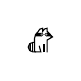
\begin{tikzpicture}[scale = 0.02]
    \draw (0,0) -- (0,8.5) arc[start angle = 180, end angle = 123.4, radius = 5.2];
    
    \draw (0,0) -- (4,0) -- +(105:4);
    \draw (6,-0.4) -- (6,5);
    \draw (8,-0.4) -- (8,7.5) -- + (30:4) -- (8, 13) -- (8,15) arc[start angle=90, end angle = 160,radius=3] -- (5.15,15) arc[start angle=90, end angle = 165,radius=3];
    
    \fill (10,8.8) arc[start angle = 215, end angle = 45, radius = 0.9];
    
    \draw (1,0) -- (0,0) -- (-1,0) arc[start angle=270, end angle=90, radius=3] -- (0,6);
    
    \fill (-1.7,0) -- (-1.7,6) -- (-0.7,6) -- (-0.7,0);
    \fill (-3.2,1) -- (-3.2,5) -- (-2.3,5.8) -- (-2.3,0.2);
    

\fill (0.2,9.9) -- (4.7,9.9) -- (4.7,12.1) -- (1.4,12.1);

\fill    (10.65,9.9) -- (7.3,9.9) -- (7.3,12.1) -- (9,12.1);


    
    \fill (7.3,11) circle[radius=1.1];
    \fill (4.7,11) circle[radius=1.1];
    \fill[white] (7.5,11) circle[radius=0.6];
    \fill[white] (4.5,11) circle[radius=0.6];
    
    \fill (7.4,11) circle[radius=0.2];
    \fill (4.4,11) circle[radius=0.2];
    
    \end{tikzpicture}



\end{document}